\label{sec:c}
The LEG controller maintains the flags and status register and handles control flow of the datapath.
The controller has the same pipeline stages as the datapath, but most signals are generated in the Decode stage. 
These signals then advance through the processor in step with the corresponding instruction.

\subsection{Relevant Files}
\begin{tabular}{|l|p{120mm}|}
\hline \textbf{File}  & \textbf{Description} \\ 
\hline controller.sv & Contains instruction decode logic to control datapath flow. Also includes micro operation state machine, exception handler, and program status registers.\\ 
\hline micropsfsm.sv & Mealy finite state machine that decodes complex instructions into sequences of simpler instructions. The instruction output by this module is used in the remaining controller decode logic.\\ 
\hline shift\_control.sv & Selects shift types, decodes shift amount, and determines shifter carry out from datapath barrel shifter. \\ 
\hline alu\_decoder.sv & Generates control signals for the ALU operation, inputs, and flags.\\
\hline memory\_mask.sv & Generates memory mask for storing different subsets of complete data words. \\
\hline conditional.sv & Checks conditional execution and kills writeback signals if an instruction should not be executed. Also generates the resultant flags of an instruction.\\
\hline exception\_handler.sv & A Mealy state machine that choreographs stalls, flushes, and branching when interrupts or exceptions are detected.\\
\hline cpsr.sv & Contains current and saved program status registers. Handles flag updates and verifies mode changes. \\
\hline 
\end{tabular} 


\subsection{Pipeline stages}
The controller Decode stage receives an instruction from the micro op FSM and generates datapath control signals.
Many control signals are needed for the execute, memory, and writeback stages. 
These are pipelined to follow the corresponding instruction, including any flushes or stalls.

Conditional execution is checked in the Execute stage.
If an instruction fails the condition check it continues to propagate through the datapath but all writeback and forwarding signals are killed. 
Thus the instruction has no effect on processor state.

\subsection{CPSR and Flags}
After a CPSR update the new flags and mode bits are forwarded to the next instruction before propagating to the writeback stage. 
The pipeline is also stalled as necessary so that the correct registers are read after any mode change.
This ensures correct operation of conditional and privileged instructions.

\subsection{MicroOp State Machine}\label{sec:uop}

The micro operation state machine is responsible for decoding complex instructions into sequences of simpler instructions. 
It takes the fetched instruction as input and outputs the instruction that is used in the rest of the processor logic. 
Additionally, the state machine outputs extra signals to enable special functionality of some instructions, such as preserving a carry bit from a previous micro op stage. 
The state transition diagram and instruction outputs of the micro op state machine is shown in Figure \ref{fig:uopdiagram}.
Table \ref{table:uops} lists the number of instructions issued for most micro operations.

\begin{figure}[h!]
\centering
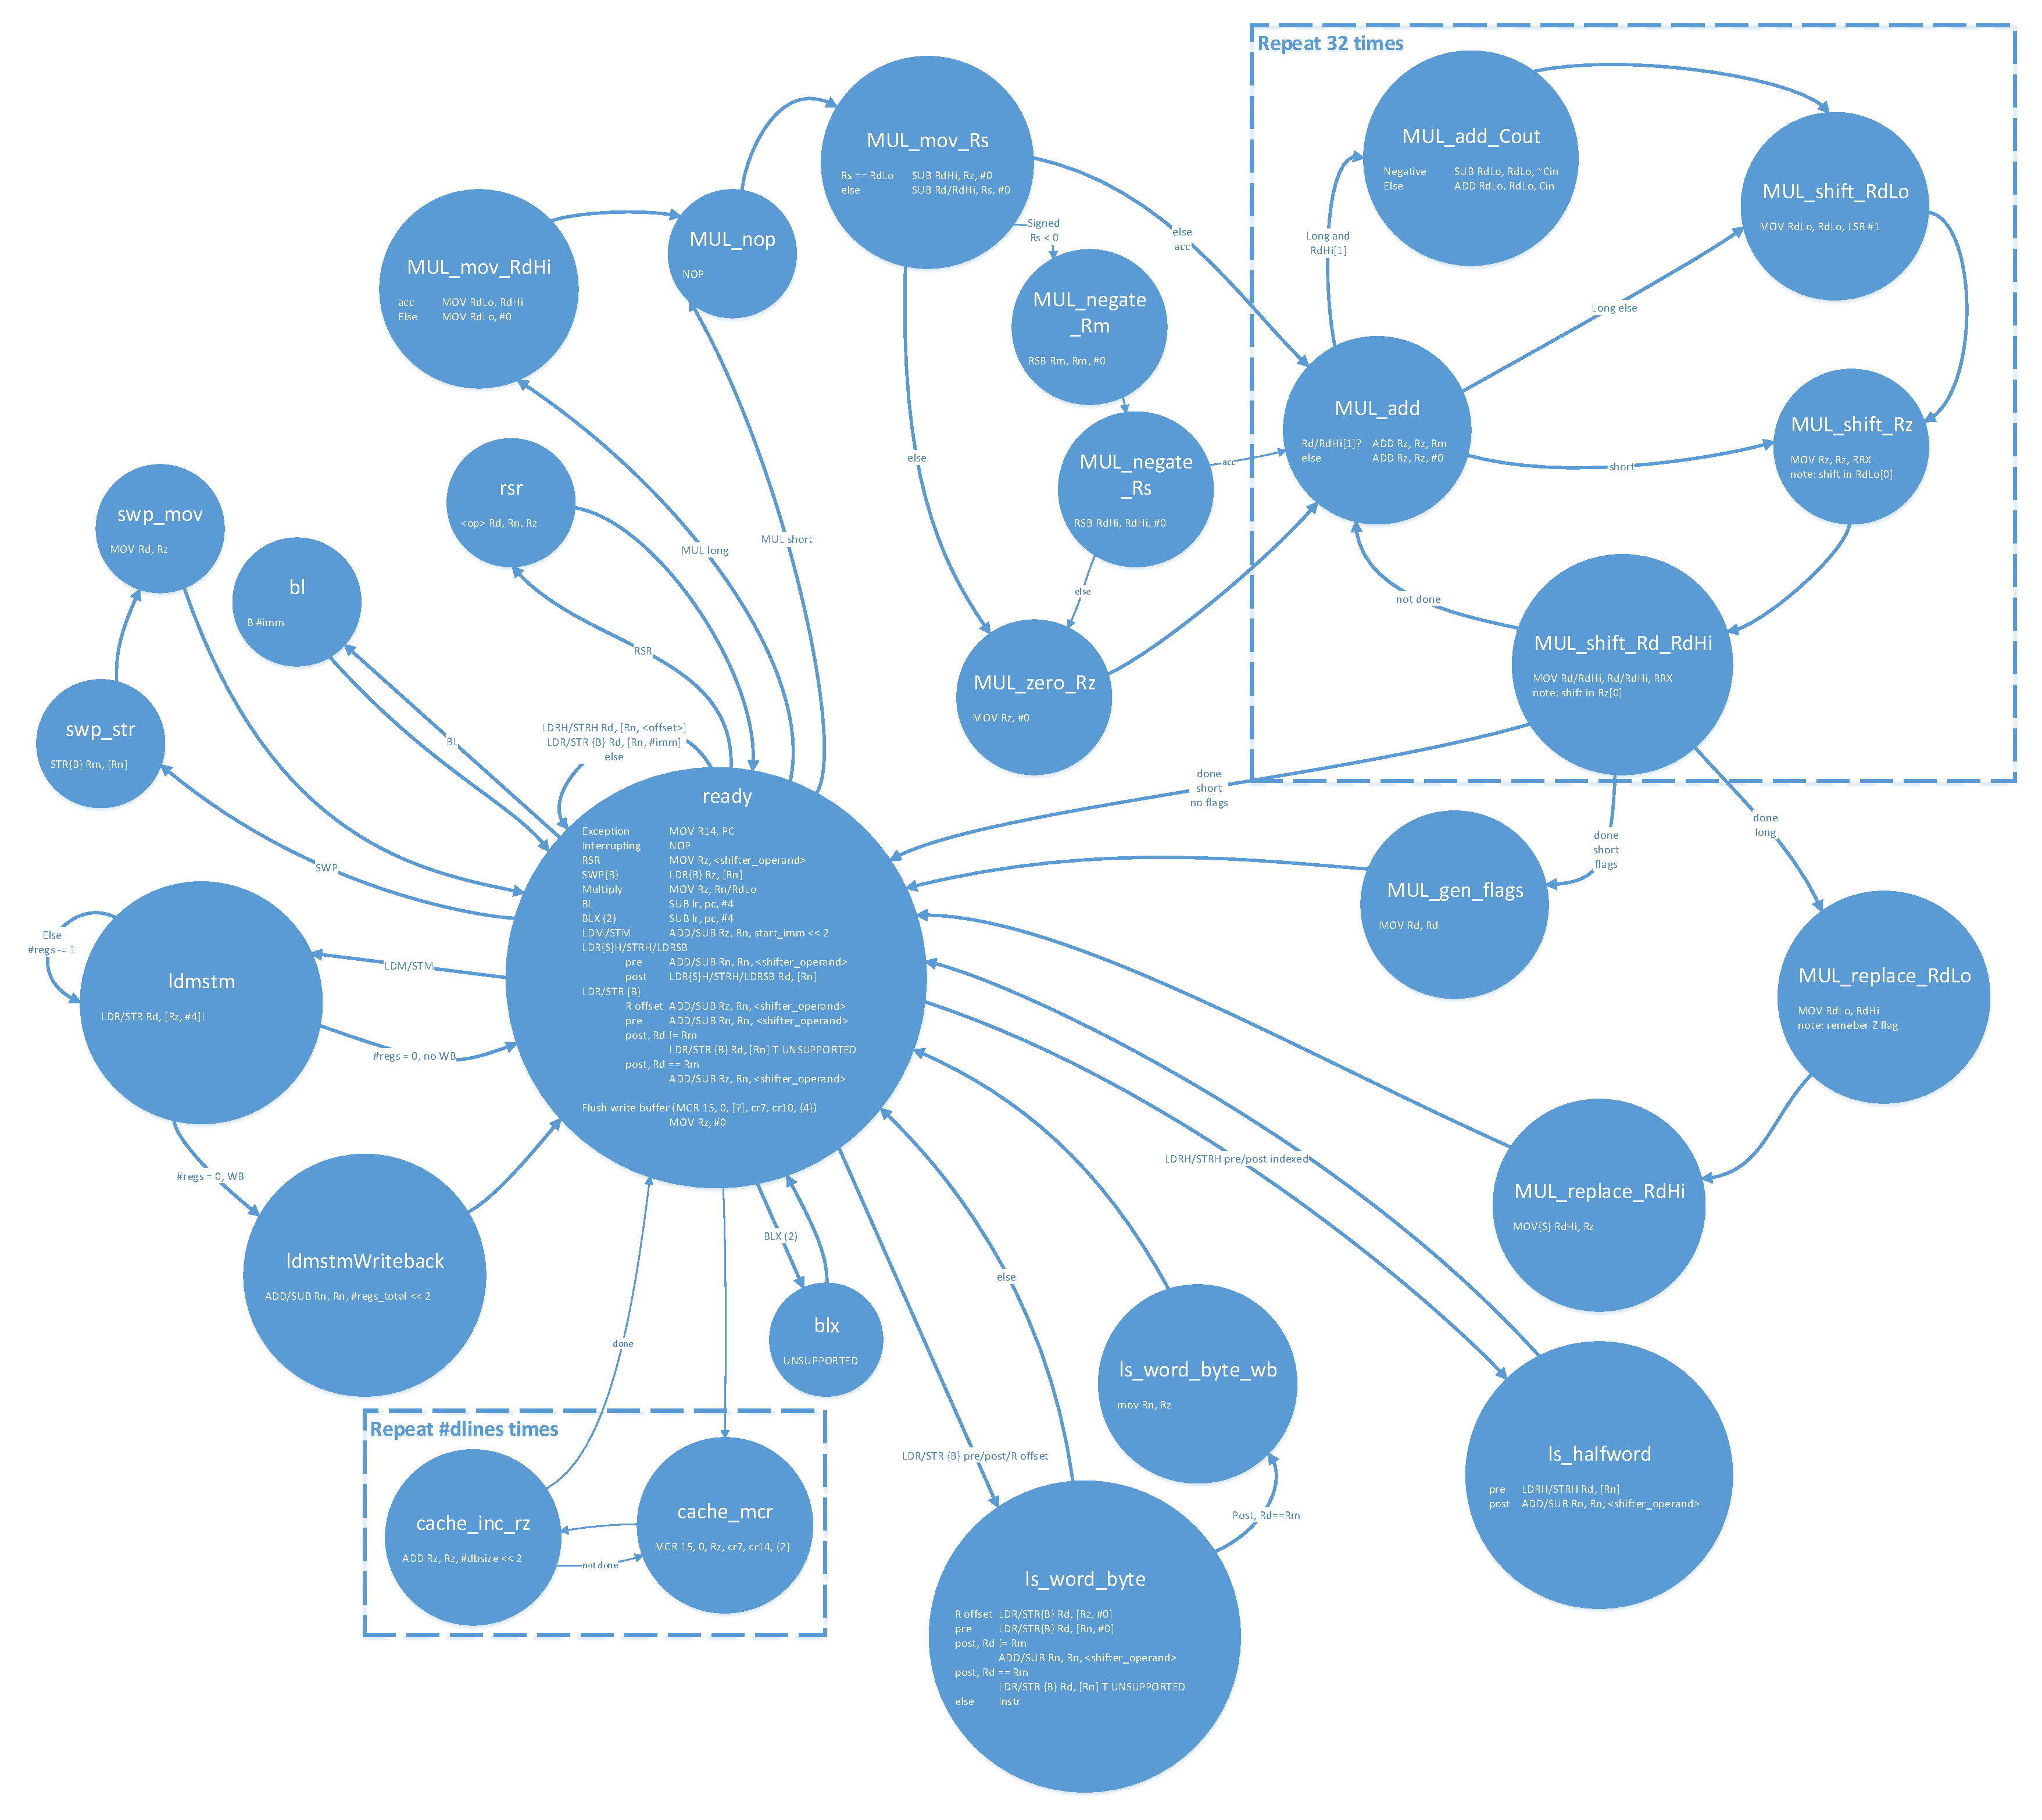
\includegraphics[width=\textwidth]{./diagrams/micropfsm_drawing.pdf}
\caption{State transition diagram for the micro op state machine. A high quality PDF is available as \texttt{documentation/diagrams/micropfsm\_drawing}}
\label{fig:uopdiagram}
\end{figure}

\begin{table}[h!]
\centering
\begin{tabular}{|l|l|}
\hline
\textbf{Instruction} & \textbf{Operations}\\
\hline
Exception & 1\\
\hline
Write buffer flush & 2 x \#dlines + 1\\
\hline
LDRH / STRH & 1-2\\
\hline
LDR / LDRB / STR / STRB & 1-3\\
\hline
Register shifted register & 2\\
\hline
BL / BLX & 2\\
\hline
SWP / SWPB & 3\\
\hline
LDM / STM & 2-18\\
\hline
MUL / MLA & 98-100\\
\hline
UMULL / UMLAL & 133-166\\
\hline
SMULL / SMLAL & 135-168\\
\hline
\end{tabular}
\caption{Number of micro-operations corresponding to each complex instruction}
\label{table:uops}
\end{table}



\subsection{Exception Issue State Machine}

The LEG exception handler is implemented as a state machine that allows interrupts and exceptions to be prioritized. 
When exceptions are detected the state machine allows the instructions before the exception-generating instruction to finish propagating through the pipeline but blocks any further instructions. 
Once the final pre-exception instruction has completed Writeback the state machine triggers saving of the program counter, mode switching, and branching to the configured exception vector.
This delay is necessary because pre-exception instructions may change the processor state including the behavior of the exception.
